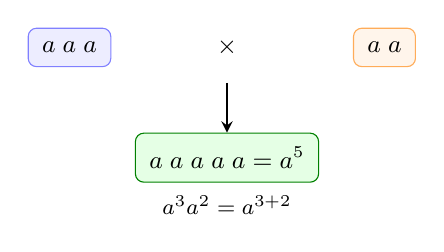
\begin{tikzpicture}[font=\small,>=stealth]
        \node[draw=blue!50,fill=blue!7,rounded corners=3pt,inner sep=5pt] (a) at (0,0) {$a\;a\;a$};
        \node[draw=orange!65,fill=orange!8,rounded corners=3pt,inner sep=5pt] (b) at (4,0) {$a\;a$};
        \node at (2,0) {$\times$};
        \node[draw=green!50!black,fill=green!10,rounded corners=3pt,inner sep=5pt] (c) at (2,-1.4) {$a\;a\;a\;a\;a=a^5$};
        \draw[->,thick] (2,-0.45)--(c.north);
        \node[font=\footnotesize] at (2,-2.0) {$a^3a^2=a^{3+2}$};
    \end{tikzpicture}
